\documentclass[11pt]{article}
\usepackage[dvipsnames]{xcolor}
\usepackage{enumitem}
\usepackage{listings}
\usepackage[listings]{tcolorbox}
\usepackage{alloy}
\usepackage{tikz}
\usepackage{url}
\usepackage{pythonhighlight}

%\usepackage{algorithm2e}
\usetikzlibrary{arrows,automata,shapes}
\tikzstyle{block} = [rectangle, draw, fill=blue!20, 
    text width=5em, text centered, rounded corners, minimum height=2em]
\tikzstyle{bt} = [rectangle, draw, fill=blue!20, 
    text width=4em, text centered, rounded corners, minimum height=2em]

\lstset{ %
basicstyle=\small\ttfamily,commentstyle=\itshape,showstringspaces=false,breaklines=true,numbers=left}
\newtcbinputlisting{\codelisting}[3][]{
    extrude left by=1em,
    extrude right by=2em,
    listing file={#3},
    fonttitle=\bfseries,
    listing options={basicstyle=\ttfamily\footnotesize,numbers=left,language=Java,#1},
    listing only,
    hbox,
}
\lstdefinelanguage{JavaScript}{
  keywords={typeof, new, true, false, catch, function, return, null, catch, switch, var, if, in, while, 
do, else, case, break},
  keywordstyle=\color{blue}\bfseries,
  ndkeywords={class, export, boolean, throw, implements, import, this},
  ndkeywordstyle=\color{darkgray}\bfseries,
  identifierstyle=\color{black},
  sensitive=false,
  comment=[l]{//},
  morecomment=[s]{/*}{*/},
  commentstyle=\color{purple}\ttfamily,
  stringstyle=\color{red}\ttfamily,
  morestring=[b]',
  morestring=[b]''
}


\newtheorem{defn}{Definition}
\newtheorem{crit}{Criterion}

\newcommand{\handout}[5]{
  \noindent
  \begin{center}
  \framebox{
    \vbox{
      \hbox to 5.78in { {\bf Software Testing, Quality Assurance and Maintenance } \hfill #2 }
      \vspace{4mm}
      \hbox to 5.78in { {\Large \hfill #5  \hfill} }
      \vspace{2mm}
      \hbox to 5.78in { {\em #3 \hfill #4} }
    }
  }
  \end{center}
  \vspace*{4mm}
}

\newcommand{\lecture}[4]{\handout{#1}{#2}{#3}{#4}{Lecture #1}}
\topmargin 0pt
\advance \topmargin by -\headheight
\advance \topmargin by -\headsep
\textheight 8.9in
\oddsidemargin 0pt
\evensidemargin \oddsidemargin
\marginparwidth 0.5in
\textwidth 6.5in

\parindent 0in
\parskip 1.5ex
%\renewcommand{\baselinestretch}{1.25}

\begin{document}

\lecture{5 --- January 19, 2026}{Winter 2026}{Patrick Lam}{version 3}

We've talked about the notion of a \emph{software failure}. Recall
that failures are caused by a \emph{fault} in the software which is executed
and whose effect propagates to output.

\section*{The Oracle Problem}

OK, so you're running your software, and you get some output. But, who's to say that the output is correct or incorrect?

The \emph{oracle problem} is: given an input and an output for a software system, determine whether or not the output is correct.

See~\cite{barr15:_oracl_probl_softw_testin} for an exhaustive survey of the research literature on the oracle problem as of 2015.

One can say ``ask a human'', but let's think some more about that.

It really is begging the question, in the strict sense of the term,
but I've been known to just take the system's output as being correct when writing
test cases.  If we're doing that, what we're doing boils down to regression testing
(depending on how critically we consider the output).

More fundamentally, though, how should the human know what correct
behaviour is? The human doesn't have any magic way of judging correctness.
They are just a human, like you or me.

This one seems easy:
\begin{lstlisting}[language=Python]
def add(x,y):
  return x + y
\end{lstlisting}
Everyone will agree\footnote{JavaScript chooses chaos for \texttt{"3"+5}.} that \texttt{add(1,1)} should return 2.

Now, let's consider root-finding. You have a function \texttt{solve\_quadratic()} which solves quadratic equations and you want to test it. If you give it $x^2 - 2x - 4 = 0$, how do you know what answer to test for? You need to read the function name and remember high school math. Also, there are the usual edge cases:
what should happen if there are no solutions? (Also, don't forget floating-point issues e.g. with comparisons.)

As a human oracle, at a unit test level, you are using the function/class name as the specification. Maybe you also consider the code documentation, if it exists.
At all levels, you combine the information that you have with your human experience. Hopefully it is reflective of the user base.

\section*{Helping Human Oracles}
Later today, we'll talk about some ways that we can
otherwise calculate the right answer, but sometimes there is
no alternative to a human looking at the test case and deciding
whether it is correct or not, as discussed just above. It comes down to whether the output
meets its requirements. Eliciting the requirements is a whole other course.

In terms of helping humans find the right answer, the literature talks about making automatically-generated inputs easier to understand, e.g. in~\cite{mcminn10:_reduc_qualit_human_oracl_costs}.

For instance, if you are testing a function that computes the days between two dates, you can easily manually evaluate the number of days between 12/24/2025 and 12/25/2025. But if one of your inputs is -5455/23195/-30879, that's going to be hard to calculate. (The function under test---not shown---sanitizes invalid inputs so that date gets parsed as 1/31/-30879, but is that a leap year?).

The suggestion is instead to generate inputs that fit expected input
profiles.  One might start from inputs that developers use as sanity
checks. (You sanity check your code, right?) Other helpful hints when
creating profiles include sanitizing checks inside the code and
variable names.  For instance, common knowledge is that valid values
for months are between 1 and 12; one can test valid values, 0,
negative values, and a value greater than 12.

There's more in~\cite{mcminn10:_reduc_qualit_human_oracl_costs} about
searches starting from normal inputs, genetic algorithms, and generating
from distributions.

Concretely, it's also possible to reuse partial inputs. This makes sense
from a testing point of view too. Change one thing at a time---it is easier
to reason about the change in the output given a single change in the input.
Go from input 11/15/2010 to 11/16/2010.

One more comment here. Sensible strings are harder to generate automatically
than numbers, since the space of strings is bigger and the space of
sensible strings is proportionately smaller. Random strings are good as
fuzzed inputs, but you also want strings that pass sanity checks. One can
mine the web for strings, or generate strings using metaheuristics
(or, these days, LLMs, I guess).

\paragraph{Crowdsourcing.} People have tried to ask Mechanical Turk
for the right answer, but apparently it's hard.

\paragraph{Reducing the volume of work for human testers.}
There's what seems to me like the eternal dream of test suite
reduction---running only the ``most important'' tests to save
execution time, and getting a good approximation to the real answer.
As far as I'm aware of, there are no good general-purpose solutions.
Test case reduction is a related concept; we'll talk about it in the
fuzzing module.

\section*{Implicit Oracles}
Segfaults are always bad. The easiest way to label a test execution as
incorrect is when it exhibits a segfault during execution.  Same
with buffer overflows, though you might need a tool to observe those.

An \emph{implicit oracle} is one that relies on implicit information
about an execution's correctness. An example of implicit information
is what we've seen above: ``segfaults are always bad''. Most implicit
oracles declare certain executions to be bad. In general, you don't
need to know anything about the domain or the specification when
labelling using an implicit oracle. Unfortunately, though, these
implicit oracles also don't give definitive evidence that the system
under test is correctly computing a result.

Other types of crashes are also most often incorrect (though an uncaught exception may be better than silently failing).  Similarly, livelock,
deadlock, and race conditions are undesirable.  Memory leaks and
performance degradations (with respect to a baseline) are other things
that can be automatically detected.

Implicit oracles and assertions are key when fuzzing---since the inputs
are automatically generated at high volume, there is going to be no
way to check that the outputs are correct. We can only check that the
outputs don't break assertions and don't crash the program.

\section*{Specification-based Oracles}
What should an implementation do? Well, one can use a
\emph{specification} to specify what the implementation should do. A
specification is some sort of description of a part of a system,
and so a \emph{specification-based oracle} is one that uses a specifcation
to declare behaviours as correct or incorrect.
Let's make that a bit more specific.

\paragraph{Model-based specification.}
There are a lot of modelling languages out there, which one
can use to describe (aspects of) system behaviour more or less formally
(depending on the language). Specifically, for a model-based specification,
one creates a model of system state, typically using sets or relations, and then
specifies operations that modify the modelled state.

Here's an example of an action predicate written in the Alloy
modelling language\footnote{\url{https://practicalalloy.github.io/chapters/behavioral-modeling/index.html}}.
\begin{lstlisting}[language=alloy]
  pred upload [f : File] {
    f not in uploaded          // guard
    uploaded' = uploaded + f   // effect on uploaded
    trashed' = trashed         // no effect on trashed
    shared' = shared           // no effect on shared
  }
\end{lstlisting}
Elsewhere in the model, we have declared sets of uploaded, trashed,
and shared files. Here, we're saying that the upload action has a
precondition that file \texttt{f} not previously be uploaded,
and that it is uploaded after completion of the action. Also,
the trashed and shared sets remain unchanged after the action.
(Alloy models can also express invariants.)

One can then use the model/specification to write test cases
which verify the specified behaviour, and test implementations using
these test cases:
\begin{itemize}[noitemsep]
\item try to upload an already-uploaded file;
\item when uploading a new file, check that the file ends up in the uploaded set, checking that trashed and shared remain the same.
\end{itemize}
The action predicate is saying what the result of the action is supposed to be---it acts as an oracle.
Models can also be verified for internal consistency.

The model uses sets, while a real implementation might use a container data structure---when writing the test case, one has to convert from specification terms to implementation terms.

\paragraph{Modelling in the implementation language.}
The model above used abstract sets.
To some extent, it is possible to specify properties using objects in the
implementation langauge.

For a filesystem that lives on the disk,
this may be difficult: there may not be an in-memory data structure that
represents the set of trashed files.

But other times, instead of using sets, the programmer can simply use
the program state to specify program properties, and express them
using assertions.  Preconditions, postconditions, and invariants can also be
specified that way, although some conditions are difficult to
efficiently verify---for instance, that a linked list is acyclic.
Some languages have specialized syntax for specifying preconditions,
postconditions, and invariants, but they can be compiled down to assertions
inserted in the appropriate places. 

\begin{lstlisting}[language=Python]
# partially self-verifying appendToList implementation
def appendToList(l,elem):
  l.append(elem)
  assert elem in l
\end{lstlisting}

Assertions can serve as explicit oracles, in contrast to the implicit
oracles we talked about above. You write a test case that arranges and acts,
but if your system under test contains assertions, then you have some explicit oracles
embedded in the code. Just like the implicit oracles, if an
assertion fails, then we know that this is a test case failure. There
is a bit more assurance in the event of an assertion success, but
I'd feel better about tests derived from model-based specifications.

\paragraph{State Transition Systems.} At some level, this is similar
to model-based specification, except that there is a finite state machine
which describes the overall system state. Wikipedia provides the turnstile example\footnote{By Chetvorno - Own work, CC0, \url{https://commons.wikimedia.org/w/index.php?curid=20269475}}:

\begin{center}
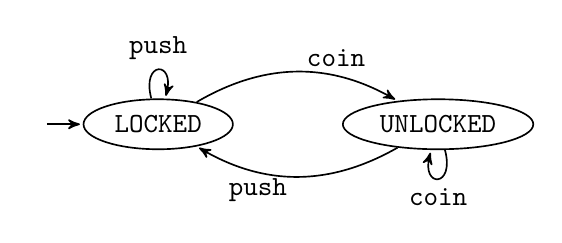
\begin{tikzpicture}[->,>=stealth',shorten >=1pt,auto,node distance=2.5cm,
                    semithick,initial text=]

  \node[initial,ellipse,draw]   (A)              {\texttt{LOCKED}};
  \node[ellipse,draw]           (B) [right of=A,xshift=3em] {\texttt{UNLOCKED}};
  
  \path (A) edge[bend left]              node[right,yshift=.5em] {\texttt{coin}} (B)
        (B) edge[bend left]              node[left,yshift=-.5em] {\texttt{push}} (A)
        (A) edge[loop above,min distance=5mm]              node {\texttt{push}} (A)
        (B) edge[loop below,min distance=5mm]              node {\texttt{coin}} (B);
\end{tikzpicture}
\end{center}

One can use the FSM as a test oracle; inserting a coin in a locked turnstile
should result in a turnstile in unlocked state. Exercise: write a test case that
expresses that idea.

\section*{Derived Test Oracles}
What about when there are no specifications, or the specifications are insufficient or unhelpful? (As you may have noticed, this is the most common case).
Here are some options, which all fall under the category of \emph{derived test oracles}.

\paragraph{Pseudo-oracles.} Consider a straightforward implementation
computing Fibonacci numbers imperatively:

\begin{python}
def fib_imperative(n):
    a = 1
    b = 1
    next = b  
    count = 1
    seq = [1, 1]

    while count <= n:
        count += 1
        a, b = b, next
        next = a + b
        seq.append(next)
    return seq
\end{python}

Of course, we can also implement Fibonacci recursively, though
it's inefficient.
\begin{python}
def fib_recursive(n):
    if n == 0:
        return 0
    elif n == 1 or n == 2:
        return 1
    return fib(n-1) + fib(n-2)
\end{python}
This is two versions. (OK, they don't provide exactly the same API.)
If they don't match, then at least one of them is wrong.

$N$-version programming extends that.
In any case, we can vote on the most popular answer between different
versions to get a ``right'' answer. It's sort of an oracle, though
if all of the versions are programmed to the wrong specification,
we still lose.

A \emph{pseudo-oracle}, then, uses a different implementation
(or implementations) as oracle(s) for the system under test.

\paragraph{Regression testing.} As mentioned earlier, regression
testing uses an earlier version as an oracle. A perfective change
in the software may require the right answer to be corrected, because
the previous version was wrong. Perhaps
the software's specifications have changed.

\paragraph{Textual documentation.} Text can also serve as a source
of truth. Usually, text requires humans to decipher it and convert it
into specifications, and then the human can either serve as a human
oracle, or the specification they write can serve as a
specification-based oracle. Maybe you can use LLMs to read text.  I
generally trust nothing coming from an LLM.

\paragraph{Specification mining.} There is work on automatically
deriving specifications from program executions, both in the form
of invariants and more general specifications. We won't go into that.

\paragraph{ECE653 note.} I am thinking of having an ECE653-only
question on the midterm where I ask specific questions which can be answered based on the 
survey~\cite{barr15:_oracl_probl_softw_testin}.

\section*{Metamorphic Testing}
We've just talked about the oracle problem---how it's difficult to know
what is the right answer for a test input.

One proposed approach to getting around the oracle problem is via
\emph{metamorphic testing}.
Sometimes we just don't have an oracle, but we want to run zillions of test cases,
and we'd like to know something about whether the output is correct or not---we want to
do better than just checking that the program doesn't crash.

The original reference to metamorphic testing is \cite{chen98:_metam}; but \cite{segura18:_metam_testin_restf_web_apis} is a more modern reference,
and contains Web examples like those in the assignment.
And, maybe a better writeup than mine by Hillel Wayne: \url{https://www.hillelwayne.com/post/metamorphic-testing/}.

The general idea is that we can run the program a bunch of times. We control the parameters
and so we can craft related inputs, such that the outputs have to be related in a certain way.
Metamorphic testing is always domain-specific, so we'll need to provide concrete examples.

\paragraph{Example: min.} Consider, then,
\begin{python}
def min(a,b):
    if a < b:
        return a
    else:
        return b
\end{python}
Let's suspend disbelief and say that we don't have an oracle for this function.
But, we know that $\mathrm{min}(a, b) = \mathrm{min}(b, a)$ should hold.
So if we have any input for $\mathrm{min}(a, b)$, say $(3, 5)$, then we can create
another input, $(5, 3)$, and we know that the result on both of these inputs should be equal.

Let the function you're testing be $f$. Three observations:
\begin{enumerate}[noitemsep]
\item if you have one input $x_0$, you can generate another input $x_1$;
\item you only know (properties of) the second expected output $f(x_1)$ in terms of the first actual output $f(x_0)$---you don't need to have a way of calculating the correct $f(x_1)$;
\item you don't necessarily know what $f(x_0)$ should be either.
\end{enumerate}
So, you can randomly generate 1 zillion test inputs for $\mathrm{min}$.
By assumption, you don't know what the corresponding outputs should be, just that
$\mathrm{min}$ shouldn't crash (implicit oracles from last time).

You can, however, given your 1 zillion test inputs, generate a second zillion test cases,
by inverting the parameter order. And you also know that the inverted test case should produce
the same output as the original test case, and you can assert on that. Well, that's something, which is better than nothing.

\paragraph{Example: search engine.}
One can argue that of course one knows what $\mathrm{min}$ should return.
It's a contrived example. Here's a less contrived example. Consider a search
engine. You can ask it a query $q$. What's more, you can ask
it for all matches of $q$ which do not contain word $w$.
Clearly, the number of hits for $q$---call that $\mathit{Count}(q)$
should be no less than the number of hits for $q$ excluding $w$---call that
$\mathit{Count}(q-w)$.
In \cite{segura18:_metam_testin_restf_web_apis}, they propose that
searching for ``metamorphic'' may return 3.3K results. If searching for
all pages with ``metamorphic'' but not containing ``testing'' returns 4.2K results,
then something is wrong. There can't be more results if you exclude a term!

You don't know what the right answer is, but in this example, you know that at least
one of the answers you got was wrong.

How can you use this insight to get new tests from old?

\paragraph{Example: speech-to-text.}
Here's another example, from a blogpost by Hillel Wayne. This one is harder to write
concrete code for, but you can definitely imagine it. Let's take a
step back. The situation is that you are writing an English
speech-to-text processor. You feed it an audio file, and you get text.

This is certainly much more open-ended than anything we see in this
course. I can read out something, and then compare the output to what
I expect. You can all do that. But this doesn't even come close to
covering the space of valid inputs.

(You could imagine using a system like Mechanical Turk to get people
to read known-text inputs, but it would be expensive to get thousands
of audio files. Or you can generate output with text-to-speech, but that's also
quite limited.)

On the other hand, you can download audio files from the Internet, but
what output should you expect? You don't know---there is no oracle, and it's
super expensive to use human oracles.

Let's use property testing. As usual, ``it doesn't crash on any input''
is a baseline property. The blogpost also suggests ``it doesn't turn
acoustic music into words'', but that's trickier to verify.
In any case, such properties don't really tell you that the system is working properly.

So, imagine that you have one input, and it transcribes to output \texttt{out}.
We know how to transform audio files. The examples are:
\begin{itemize}[noitemsep]
\item double the volume; or,
\item raise the pitch; or,
\item increase the tempo; or,
\item add background static; or,
\item add trafic noises; or,
\item combine any of these.
\end{itemize}
So if you take our input and apply transformations, you can still expect the transformed
audio file to transcribe to \texttt{out}. Indeed, you can take 10 different traffic noises,
and then you have 11 (10 + the original) cases to test. You can then double the volume, and
you have 22 cases. You know the correct answer for all of these, and your tests now cover much more
of the input space.

But wait, there's more. In this case, you knew the output. But you can actually run your system
on a collection of related tests without knowing the expected output. The output is supposed
to be the same on all of them, but you don't care what it is. This allows you to vastly scale
your testing to cases where you don't have an oracle: the blogpost suggests, for instance, downloading
an episode of \emph{This American Life}\footnote{Canadian content plug: The Debaters on CBC might be better: \url{https://www.cbc.ca/radio/thedebaters}} (or, all of them), transforming it, and seeing if the output
on all the transformed episodes match.

\paragraph{Example: real-life YouTube search.} 
From~\cite{segura18:_metam_testin_restf_web_apis}, here's an example from the YouTube search API
in particular. They found that a search for ``winter pentathlon 1949'' returned 15 items;
but issuing the same query and asking for ordering by date returned 0 items. That's not right\footnote{YouTube today returns things you didn't ask for.}.
Here is a figure from the paper I've cited.

\includegraphics[width=\textwidth]{L06/metamorphic-youtube.png}

\paragraph{Example: tagged image search.}
This example is the one I've put on the assignment. Maybe I can explain it more clearly this time.
Consider an image gallery, where you can tag images. Let's say that there are tags ``red'' and ``blue'',
for pictures that contain something red, or something blue, respectively. A picture may be tagged both
``red'' and ``blue''.

Let's also say that there are 4 images, numbered 1 through 4. Images \{1, 2, 3\} are tagged ``red'',
while images \{1, 2, 4\} are tagged ``blue''. There are no other images and no other tags.

If you request all images with any tag, then you'll get all 4 images: \{1, 2, 3, 4\}.

If you request all images tagged ``red'' and, separately, all images tagged ``blue'',
then you get 3 results for each of the requests. If you add $3+3$ then you get 6,
and this number 6 has to be greater than or equal to 4, the total number of images which have any tag.

Symbolically, let $T$ be the set of tags, and let $\#(S)$ count the number of images with tags in the set $S$. This has to be true:
\[ \sum_{t \in T} \#( \{ t \} ) \ge \#(T).\]


\subsection*{Metamorphic Relations}
The paper~\cite{segura18:_metam_testin_restf_web_apis} provides a list of metamorphic relation output patterns.
Here's a brief explanation.

\begin{itemize}[noitemsep]
\item Equivalence: the source and follow-up inputs produce equivalent outputs---same items, though perhaps in a different order.
  Example: source input is a query, follow-up input is the same query but with some different ordering requested, like ``sort by date''.
\item Equality: source and follow-up inputs produce equal output---same items, same order. Example: source input uses the default value,
  follow-up input specifically requests the default. Specific example: default order is relevance; initial input omits the order,
  follow-up input asks for relevance order.

  One can also have relations where the source output is equal to at least one of the follow-up outputs.
\item Subset: follow-up output is a (possibly strict) subset of the source output. Example: filtering a set of query results.
  Specific example: YouTube videos and narrowing the geolocation further between the source and the follow-up, say from 50km from
  a point to 25km to a point.
\item Disjoint: source and follow-up outputs should be disjoint. Specific example: source input = Spotify albums of ``michael buble'' from 2012,
  follow-up input = Spotify albums of ``michael buble'' from 2014. There should be no items in both output sets.
\item Complete: the union of the follow-up outputs completely make up the source output. Specific example: there are short, medium, and long YouTube
  videos. If the source input is for keyword ``testing'', then one can make three follow-up inputs: short ``testing'', medium ``testing'', and long ``testing''.
  Put together, the results for short, medium, and long ``testing'' videos should be the same as the results for just ``testing''.
\item Difference: source and follow-up differ in a specific set of items $D$. Often occur in create and update operations. Specific example:
  I upload two videos which I know to be similar except for the length and title. The create operation returns the video uploaded.
  One can check that the source and follow-up output metadata only differ on items in $D$: for instance, they should have the same resolution, but may have different length and title.
\end{itemize}

\bibliographystyle{alpha}
\bibliography{L05}


\end{document}
